Für die Bestimmung des Templates des korrelierten Untergrunds wird das Template des Signals von einer Verteilung invarianter Masse abgezogen.
Die Verteilung invarianter Masse kommt dabei aus der Monte Carlo Simulation, auf die das Analyseverfahren bis einschließlich der Abschätzung der unkorrelierten Untergrunds, so wie bisher erläutert, angewandt wurde.
\begin{figure}[tp]
\centering
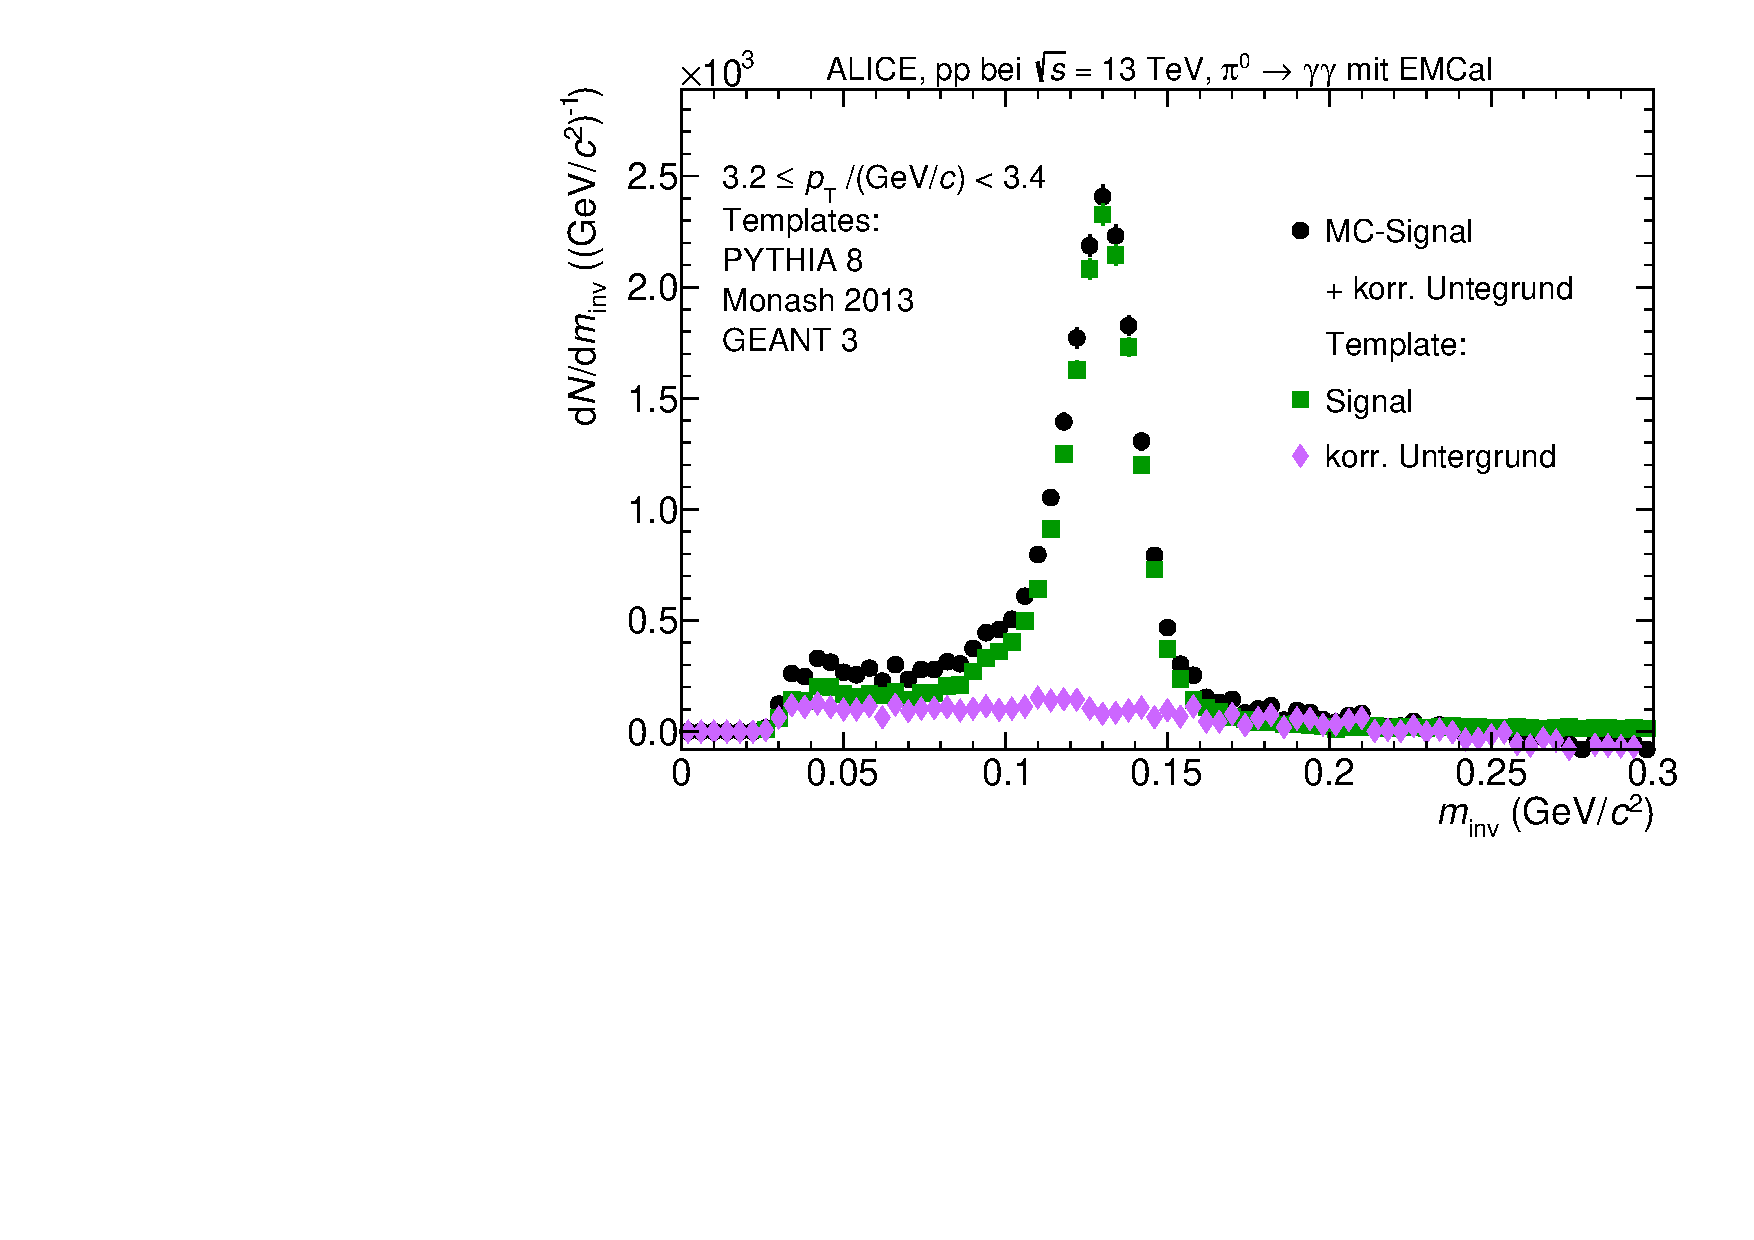
\includegraphics[width=.75\linewidth]{EntstehungUntergrund10_Data_2016.pdf}
\caption{Template des korrelierten Untergrunds in pink entstanden durch den Abzug des Templates des Signals (grün) von der Verteilung der invarianten Masse aus einer Monte Carlo Simulation (schwarz).}
\label{fig:BkgTemp}
\end{figure}
\newline
Das Template des korrelierten Untergrunds für das $p_\text{T}$-Intervall $(3\,2 - 3\,4) (\text{GeV/}c)$ wird in Abbildung \ref{fig:BkgTemp} in pink dargestellt.
Zur Verdeutlichung sind ebenfalls das oben beschriebene Signal in schwarz und das Template des Signals in grün eingezeichnet.
\newline
Für großes $p_\text{T}$ wird die Unsicherheit im Template des korrelierten Untergrunds relativ groß im Verglichen mit der Anzahl an Einträgen in der Verteilung der invarianten Masse.
Deshalb wird in dieser Arbeit der korrelierte Untergrund aus mehreren $p_\text{T}$-Intervallen zusammengefasst.
Dabei wird angenommen, dass sich nicht die Form, sondern nur die Anzahl der Einträge in den $p_\text{T}$-Intervallen unterscheidet.  
Für die Zusammenfassung der Templates des korrelierten Untergrunds werden die Templates des korrelierten Untergrunds aus den $p_\text{T}$-Intervallen von $p_\text{T} \geq 1\,8\text{ GeV}/c$ bis $p_\text{T} \leq 3\,2\text{ GeV}/c$ aufgrund der geringen statistischen Unsicherheit benutzt.
Diese werden zunächst aufsummiert und auf die Anzahl der verwendeten $p_\text{T}$-Intervalle normiert.
\begin{figure}[tp]
\centering
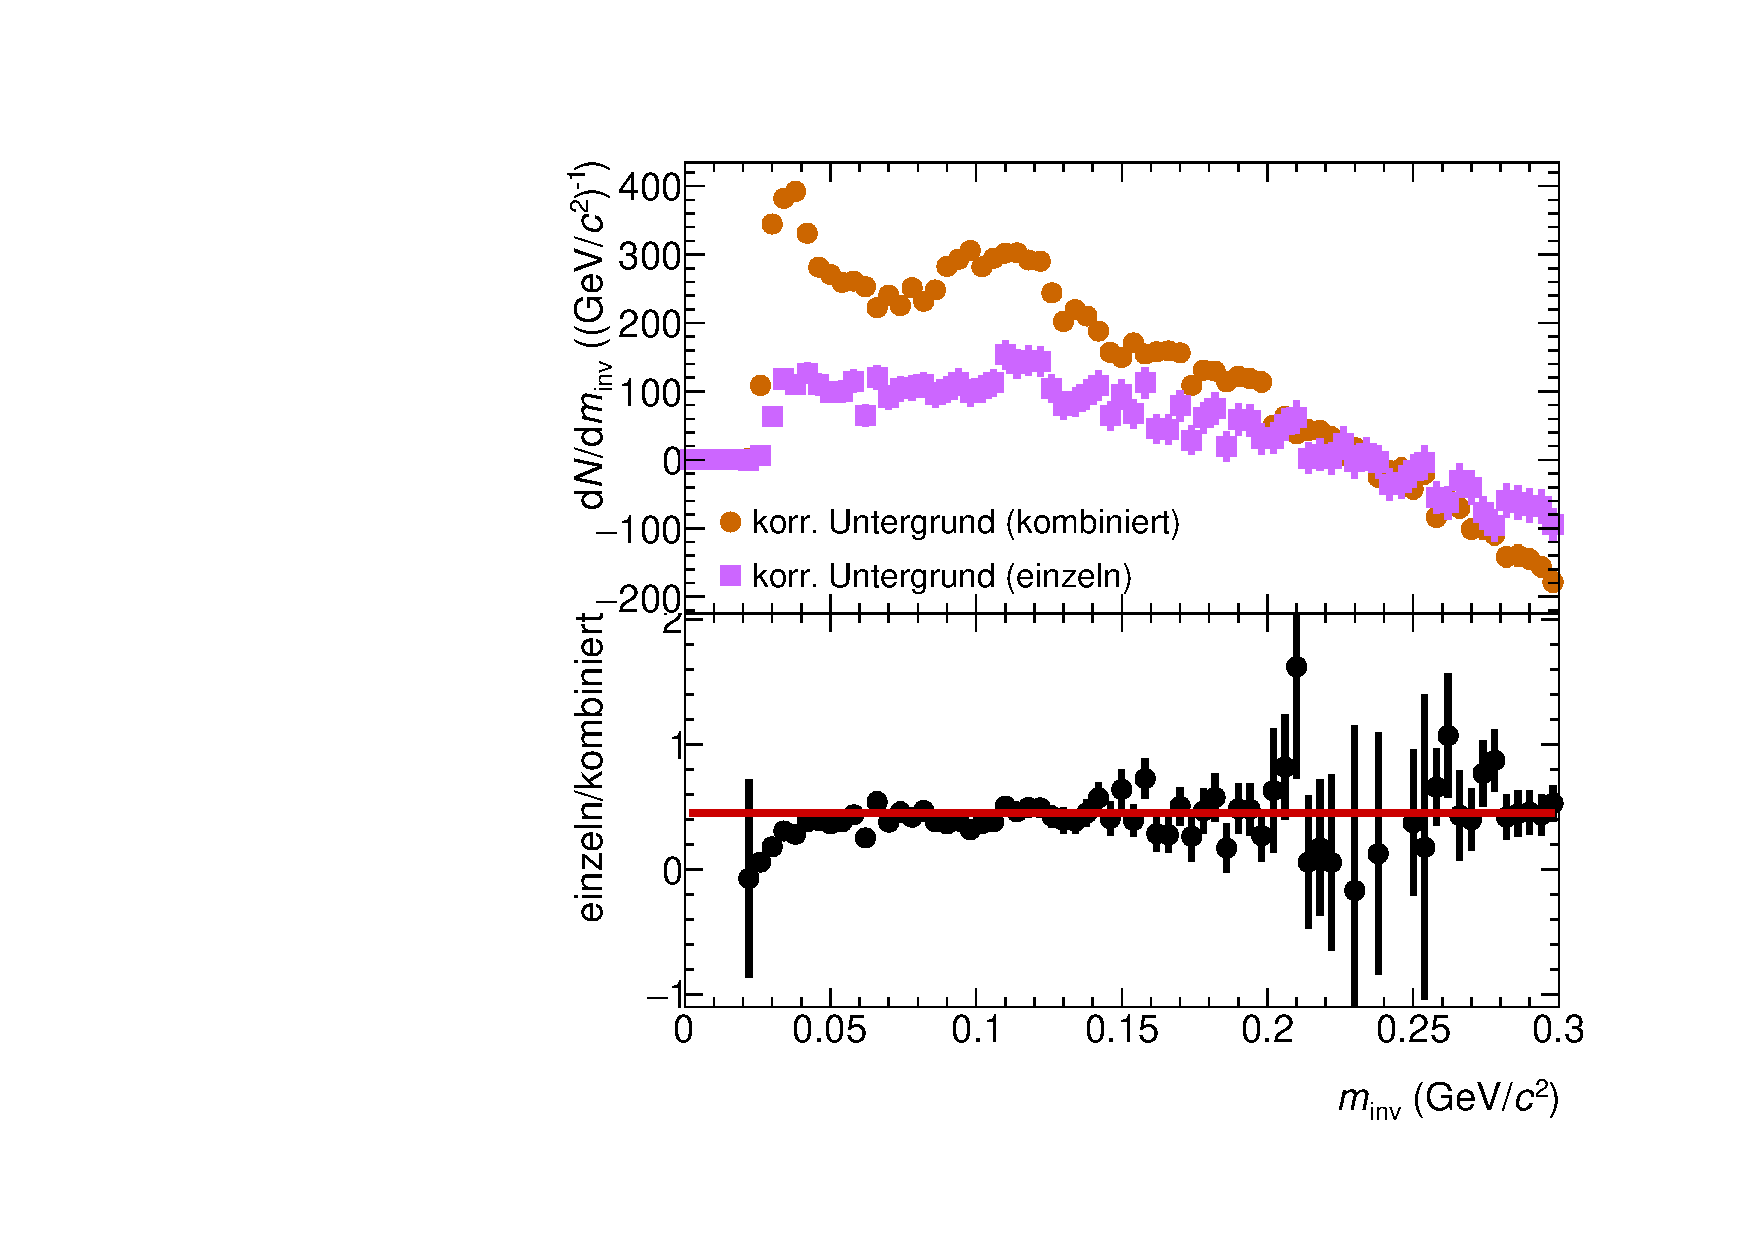
\includegraphics[width=.7\linewidth]{BackgroundWithRatio10_Data_2016.pdf}
\caption{\textbf{Oben:} Template des korrelierten Untergrunds aus einem einzelnen $p_\text{T}$-Intervall in pink und aus mehreren $p_\text{T}$-Intervallen kombiniert in orange.
\textbf{Unten:} Verhältnis der beiden Verteilungen in schwarz, sowie Parametrisierung einer Konstante an das Verhältnis in rot.}
\label{fig:BkgTempRatio}
\end{figure}
\newline
Abbildung \ref{fig:BkgTempRatio} oben in orange ein kombiniertes Template des korrelierten Untergrunds und in pink das Template des korrelierten Untergrunds für das $p_\text{T}$-Intervall $(3\,2 - 3\,4) (\text{GeV/}c)$.
Um zu zeigen, dass die Annahme ihre Richtigkeit hat wird unten das Verhältnis aus einzelnem Template des korrelierten Untergrunds zu den Kombinierten dargestellt.
Die rote Linie im unteren Teil der Abbildung basiert auf einer konstanten Parametrisierung des Verhältnisses.
Die getroffene Annahme wird bestätigt, da die konstante Parametrisierung und das Verhältnis gut miteinander übereinstimmen.
Die großen Unsicherheiten im Verhältnis um $m_\text{inv} = 0,225\text{ GeV}/c^{2}$ entsteht, da beide Templates an dieser Stelle eine Anzahl an Einträgen nah um Null besitzen.
\newline
Zuvor wurde bereits angesprochen, dass die Anforderung an den Öffnungswinkel abhängig von $p_\text{T}$ ist.
Um das kombinierte Template des korrelieren Untergrunds daran anzupassen wurde eine vereinfachte Monte Carlo Simulation durchgeführt.
Dadurch konnten größere Abweichungen für kleinere invariante Massen vermieden werden.
\newline
Später wird für die Bestimmung der systematischen Unsicherheit die Wahl des Templates des korrelierten Untergrunds variiert.
Zum einen werden die Templates einzeln verwendet, also jeweils das Template des korrelierten Untergrunds aus dem jeweiligen $p_\text{T}$-Intervall, aus dem auch die Verteilung der invarianten Masse und das Template des Signals kommen.
Zum anderen wird die Kombination variiert, sodass das Template des korrelierten Untergrunds nicht aus einem festen vergrößerten $p_\text{T}$-Intervall stammt.
Stattdessen wird das $p_\text{T}$-Intervall eines einzelnen Templates des korrelierten Untergrunds ausgeweitet, bis das Intervall mindestens $4\text{ GeV}/c$ umfasst.
\newline
Im Folgenden Abschnitt werden die beiden Templates so parametrisiert, dass sie das Signal nach Abschätzung des unkorrelierten Untergrunds bestmöglich beschreiben.